\documentclass{article}

\usepackage{graphicx}
\usepackage{tikz}
\usepackage{tikzsymbols}
\usetikzlibrary{calc,patterns,shapes.geometric}
\pagestyle{empty}
\usepackage[margin=0pt]{geometry}
\geometry{papersize={14in,12in}}

\def\centerarc[#1](#2)(#3:#4:#5){\draw[#1] ($(#2)+({#5*cos(#3)},{#5*sin(#3)})$) arc (#3:#4:#5);}

\begin{document}
	\begin{figure}
		\centering
		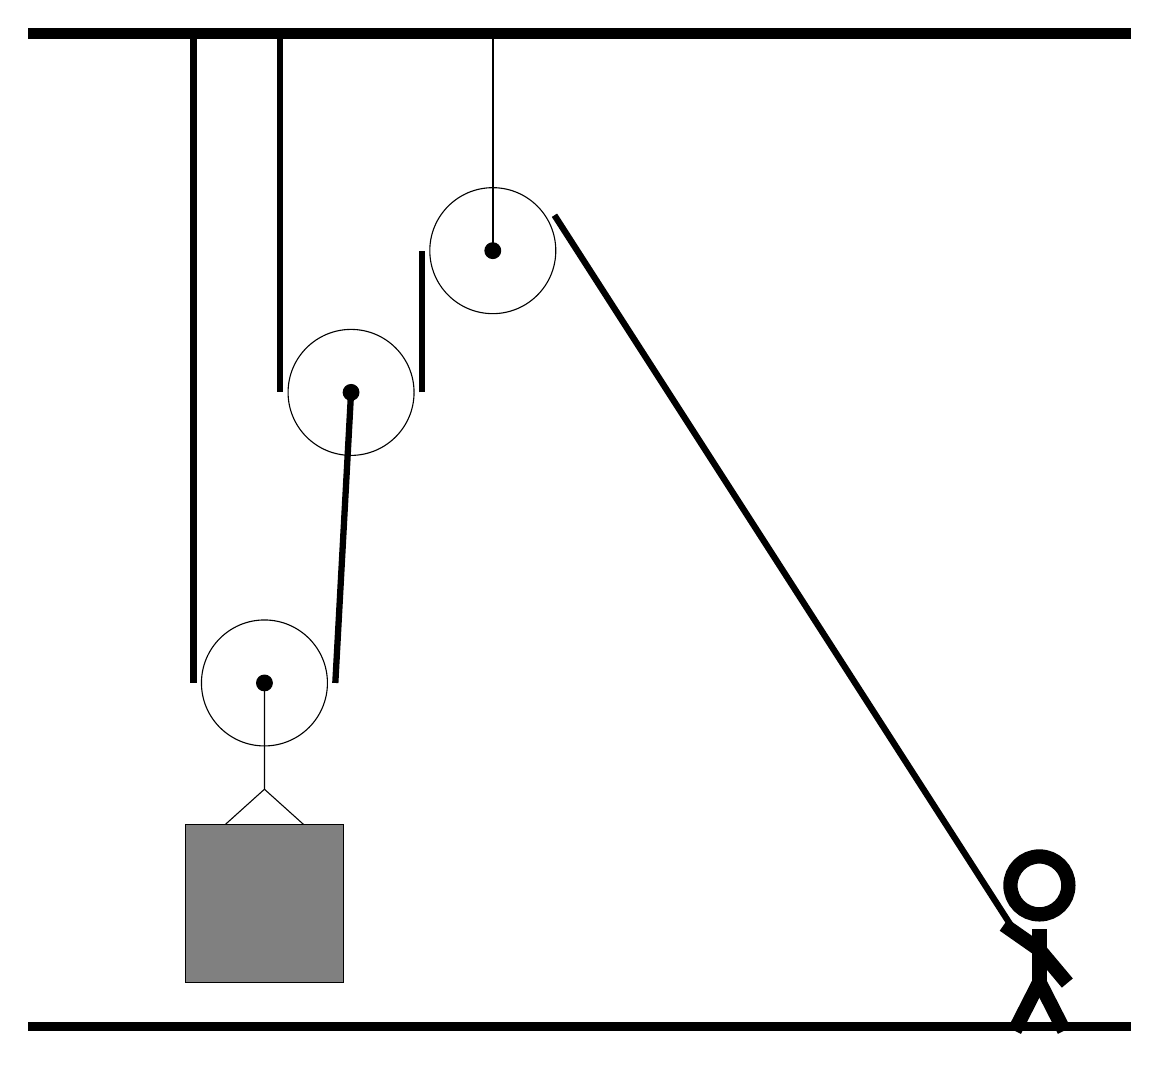
\begin{tikzpicture}
			%%%%% START %%%%%
			\draw[fill=black] (-2, 9) rectangle (12, 9.125);
			
			\draw (1, 0.81) circle (0.8);
			\draw[fill=black] (1, 0.81) circle (0.1);
			
			\draw (2.1, 4.5) circle (0.8);
			\draw[fill=black] (2.1, 4.5) circle (0.1);
			
			\draw (3.9, 6.3) circle (0.8);
			\draw[fill=black] (3.9, 6.3) circle (0.1);
			\draw[thick] (3.9, 6.3) -- (3.9, 9);
			
			\draw (1, 0.81) -- (1, -0.54) -- (0.5, -0.99) -- (1.5, -0.99) -- (1, -0.54);
			\draw[fill=black!50] (0, -0.99) rectangle (2, -2.99);
			
			\draw[line width=0.8mm] (0.1, 9) -- (0.1, 0.81);
			\centerarc[line width=0.8mm](1, 0.81)(180:360:0.9);
			\draw[line width=0.8mm](1.9, 0.81) -- (2.1, 4.5);
			\draw[line width=0.8mm] (1.2, 9) -- (1.2, 4.5);
			\centerarc[line width=0.8mm](2.1, 4.5)(180:360:0.9);
			\draw[line width=0.8mm](3.0, 4.5) -- (3.0, 6.3);
			\centerarc[line width=0.8mm](3.9, 6.3)(30:180:0.9);
			\draw[line width=0.8mm] (4.683, 6.75) -- (10.5, -2.3);
			
			\node at (10.8, -2.5) {\Strichmaxerl[10][-35][-50]};
			
			\draw[fill=black] (-2, -3.5) rectangle (12, -3.6);
			%%%%% END %%%%%
		\end{tikzpicture}
	\end{figure}	
\end{document}